\documentclass[12pt, letterpaper]{../assignment}
\usepackage{graphicx}
\usepackage{courier}
\usepackage{minted}
\usepackage{amsmath}
\usepackage{polynom}
\usepackage{commath}
\usepackage{amssymb}
\usepackage{amsfonts} 
\usepackage{color}
\usepackage{cancel}
\usepackage{enumitem}
\usepackage{graphicx}
\usepackage{multirow}
\usepackage{float}
\usepackage{bm}
\usepackage{tikz}
\usetikzlibrary{shapes,arrows}
\usepackage{booktabs}
\usetikzlibrary{patterns}

% Define Theme Colors
\definecolor{light-gray}{rgb}{0.2,0.2,0.2}
\definecolor{header-blue}{rgb}{0,0,0.7}
% \definecolor{header-blue}{rgb}{0.5137,0.8353,0.9176}
\definecolor{header-blue}{rgb}{0,0.8,0.95}
\definecolor{dark-gray}{rgb}{0.1,0.1,0.1}
\pagecolor{dark-gray}
\color{white}

\usemintedstyle{monokai}
\oddsidemargin = 0pt
\exercisesheet{Module 11}{Assignment}
\student{Austin Barrilleaux}
\university{\color{header-blue}Johns Hopkins University}
\school{\color{header-blue}Whiting School of Engineering}
\courselabel{EN 535.612}
\semester{Fall 2024}
\usepackage[backend=bibtex,style=numeric,sorting=none]{biblatex}
\bibliography{reference}

\definecolor{light-gray}{rgb}{0.2,0.2,0.2}
\setminted{bgcolor=light-gray,frame=lines,rulecolor=white}
\setlength{\parindent}{0pt}

\makeatletter
\patchcmd{\minted@colorbg}{\noindent}{\medskip\noindent}{}{}
\apptocmd{\endminted@colorbg}{\par\medskip}{}{}
\makeatother

\begin{document}

\subsection*{Problem 1: Solve Ginsberg 9.28}
\subsubsection*{The absolute velocity of a particle may be represented by the components $\bm{v_x}$,
$\bm{v_y}$, and $\bm{v_z}$ relative to the axes of a moving reference system $\bm{xyz}$.
Suppose that the angular velocity $\bm{\bar{\omega}}$ of $\bm{xyz}$ and the velocity
$\bm{\bar{v}_O}$ of the origin of $\bm{xyz}$ are known as functions of time.
Derive the Gibbs-Appell equations of motion relating the quasi-velocities $\bm{\dot{\gamma}_1 = v_x}$, $\bm{\dot{\gamma}_2 = v_y}$,
and $\bm{\dot{\gamma}_3 = v_z}$ to the resultant force acting on the particle.}

Where:

$$ \bar{\omega} = 
\left<\begin{array}{c} \omega_x \\ \omega_y \\ \omega_z \end{array}\right>  $$

Given that:

$$ \bar{v} =
\left<\begin{array}{c} v_x \\ v_y \\ v_z \end{array}\right> =
\left<\begin{array}{c} \dot{\gamma}_{1}\\ \dot{\gamma}_{2}\\ \dot{\gamma}_{3} \end{array}\right> $$ 

Solving for acceleration:

\begin{equation*}
\begin{aligned}
    \bar{a} &= \frac{\partial \bar{v}}{\partial t} + \bar{\omega} \times \bar{v} \\
            &= \frac{\partial \dot{\gamma}}{\partial t} + \bar{\omega} \times \dot{\gamma} \\
            &= \left<\begin{array}{c}
{\ddot{\gamma}}_1 -{\dot{\gamma} }_2 \,\omega_z +{\dot{\gamma} }_3 \,\omega_y \\
{\ddot{\gamma}}_2 +{\dot{\gamma} }_1 \,\omega_z -{\dot{\gamma} }_3 \,\omega_x \\
{\ddot{\gamma}}_3 -{\dot{\gamma} }_1 \,\omega_y +{\dot{\gamma} }_2 \,\omega_x 
\end{array}\right>
\end{aligned}
\end{equation*}

Given that the Gibbs-Appell function for a system of particles is:

$$ S = \sum_p \frac{1}{2} m \bar{a}_p \cdot \bar{a}_p  $$

For this single particle case:

\begin{equation*}
\begin{aligned}
S &= \frac{1}{2} m \left( \bar{a}\cdot \bar{a} \right) \\
  &= \frac{1}{2}m\,{\left[
                  {{\left({\ddot{\gamma} }_3 -{\dot{\gamma} }_1 \,\omega_y +{\dot{\gamma} }_2 \,\omega_x \right)}}^2 +
                  {{\left({\ddot{\gamma} }_2 +{\dot{\gamma} }_1 \,\omega_z -{\dot{\gamma} }_3 \,\omega_x \right)}}^2+
                  {{\left({\ddot{\gamma} }_1 -{\dot{\gamma} }_2 \,\omega_z +{\dot{\gamma} }_3 \,\omega_y \right)}}^2
                  \right]}
\end{aligned}
\end{equation*}

Where the equations of motion are calculated as:

$$ \frac{\partial S}{\partial \ddot{\gamma}_j} =
\Gamma_j = \Gamma_1 $$ %=  \sum \bar{F} \cdot \bar{v}_j(q_i,t)  $$

The virtual work associated with the forces applied to the particle is:

$$ \delta W = 
\sum \bar{F} \cdot \delta \bar{r} = 
\sum_{j1}^K
\Gamma_j\ \delta \gamma_j = %\sum \bar{F} \cdot \bar{v}_{P_j}(q_i,t)\ \delta \gamma_j  $$
\sum \bar{F} \cdot \left<\begin{array}{c}
  \delta \gamma_1 \\
  \delta \gamma_2 \\
  \delta \gamma_3
\end{array}\right> $$ 

The equation of motion is solved for as:

\begin{equation*}
\begin{aligned}
    \frac{\partial S}{\partial \ddot{\gamma}} 
      &= m\left<\begin{array}{c}
{\ddot{\gamma} }_1 -{\dot{\gamma} }_2 \,\omega_z +{\dot{\gamma} }_3 \,\omega_y \\
{\ddot{\gamma} }_2 +{\dot{\gamma} }_1 \,\omega_z -{\dot{\gamma} }_3 \,\omega_x \\
{\ddot{\gamma} }_3 -{\dot{\gamma} }_1 \,\omega_y +{\dot{\gamma} }_2 \,\omega_x 
\end{array}\right>
= \Gamma_1 = 
\left<\begin{array}{c}
  \sum F_x \\
  \sum F_y \\
  \sum F_z
  \end{array}\right>
\end{aligned}
\end{equation*}


Or:

\begin{answer}
  \begin{equation*}
    \begin{aligned}
    m\left({\ddot{\gamma} }_1 -{\dot{\gamma} }_2 \,\omega_z +{\dot{\gamma} }_3 \,\omega_y\right) &= \sum F_x \\
    m\left({\ddot{\gamma} }_2 +{\dot{\gamma} }_1 \,\omega_z -{\dot{\gamma} }_3 \,\omega_x\right) &= \sum F_y \\
    m\left({\ddot{\gamma} }_3 -{\dot{\gamma} }_1 \,\omega_y +{\dot{\gamma} }_2 \,\omega_x\right) &= \sum F_z
    \end{aligned}
    \end{equation*}
\end{answer}

Where:

  \begin{equation*}
    \begin{aligned}
      \dot{\gamma} =
      \left<\begin{array}{c} \dot{\gamma}_1 \\ \dot{\gamma}_2 \\ \dot{\gamma}_3  \end{array}\right>
      = v =
      \left<\begin{array}{c} v_x \\ v_y \\ v_z  \end{array}\right>
      = v_0 + \bar{\omega} \times \bar{r}
      = \left<\begin{array}{c}
        v_{0_x} -\omega_z \,y+\omega_y \,z\\
        v_{0_y} +\omega_z \,x-\omega_x \,z\\
        v_{0_z} -\omega_y \,x+\omega_x \,y
        \end{array}\right> 
    \end{aligned}
    \end{equation*}

Where:


\subsection*{Problem 2:}
\subsubsection*{Use the Gibbs-Appell approach to find the equations of motion for this problem.}
\subsubsection*{A torque $\bm{\Gamma}$ applied to the vertical shaft of the T-bar
causes the rotation rate $\bm{\Omega}$ about the vertical axis to increase in proportion to the angle $\bm{\theta}$ by which bar BC swings outward,
that is, $\bm{\Omega = c\theta}$.
The mass of bar BC is $\bm{m_1}$ and the moment of inertia of the T-bar about its axis of rotation is $\bm{I_2}$.
Determine the equations of motion for the system, and for the torque $\bm{\Gamma}$.}

\begin{figure}[H]
    \centering
    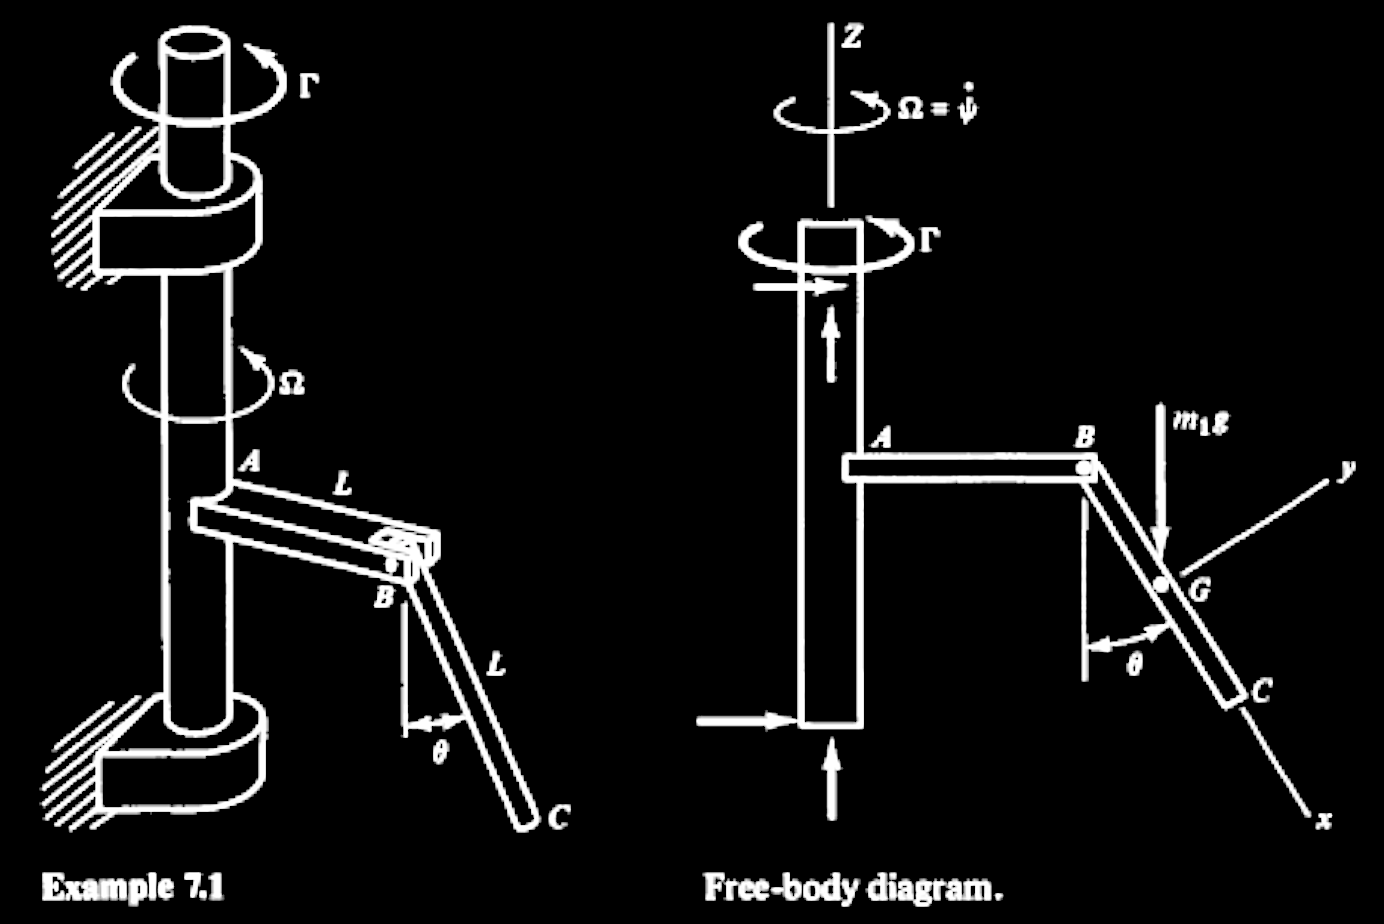
\includegraphics[scale=0.5,frame]{images/Problem_2.png}
\end{figure}

$$ \left(\begin{array}{c} \frac{L\,\cos\left(\psi \right)\,\cos\left(\theta \right)\,\frac{\partial }{\partial t} \dot{\gamma }_{1}}{2}-\frac{L\,\cos\left(\psi \right)\,\sin\left(\theta \right)\,{\dot{\gamma }_{1}}^2}{2}-\frac{L\,c^2\,\cos\left(\psi \right)\,{\theta }^2\,\left(\sin\left(\theta \right)+2\right)}{2}-\frac{L\,c\,\sin\left(\psi \right)\,\dot{\gamma }_{1}\,\left(\sin\left(\theta \right)+2\right)}{2}-L\,c\,\cos\left(\theta \right)\,\sin\left(\psi \right)\,\dot{\gamma }_{1}\,\theta \\ \frac{L\,\cos\left(\theta \right)\,\sin\left(\psi \right)\,\frac{\partial }{\partial t} \dot{\gamma }_{1}}{2}-\frac{L\,\sin\left(\psi \right)\,\sin\left(\theta \right)\,{\dot{\gamma }_{1}}^2}{2}-\frac{L\,c^2\,\sin\left(\psi \right)\,{\theta }^2\,\left(\sin\left(\theta \right)+2\right)}{2}+\frac{L\,c\,\cos\left(\psi \right)\,\dot{\gamma }_{1}\,\left(\sin\left(\theta \right)+2\right)}{2}+L\,c\,\cos\left(\psi \right)\,\cos\left(\theta \right)\,\dot{\gamma }_{1}\,\theta \\ \frac{L\,\sin\left(\theta \right)\,\frac{\partial }{\partial t} \dot{\gamma }_{1}}{2}+\frac{L\,\cos\left(\theta \right)\,{\dot{\gamma }_{1}}^2}{2} \end{array}\right) $$

% % \color{white}
% \hspace*{6em}\inputminted[frame=leftline,fontsize=\footnotesize,lastline=51]{matlab}
% {./matlab/Problem_2.m}
% % \color{black} 

% % \color{white}
% \hspace*{6em}\inputminted[frame=leftline,fontsize=\footnotesize]{matlab}
% {./matlab/Q6_8.m}
% % \color{black} 

% \begin{figure}[H]
%     \centering
%     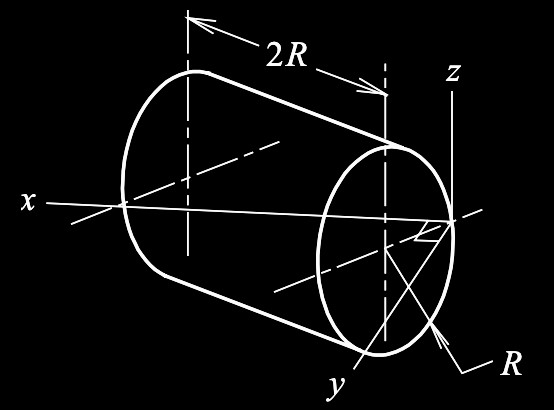
\includegraphics[scale=0.7,frame]{images/Q5_13.png}
% \end{figure}




\end{document}

